\chapter{Matematica di base}
\section{Insiemi di numeri}
I numeri sono così diffusi nel nostro mondo che si comincia a farne uno sin dai primi anni di vita. Resta tuttavia indispensabile per gli studenti che hanno deciso di intraprendere studi universitari di questo tipo, ripassare alcuni concetti. 
L’esigenza nasce dalla necessità di fare alcuni chiarimenti su alcuni aspetti delicati e profondi dei numeri che giocano poi un ruolo fondamentale in tutta la matematica.

I primi numeri che si incontrano sono gli interi positivi, detti anche numeri naturali.
\begin{center}
    $\mathbb{N} = \{0,1,...\}$
\end{center}

E’ poi conveniente anche introdurre i numeri con il segno per poter trattare grandezze negative e i numeri frazionari per misurare lunghezze, aree, temperature ...
Da qui nasce la necessità di introdurre due nuovi insiemi. I numeri interi e quelli razionali.
\begin{center}
    $\mathbb{Z} = \{...,-1,0,1,...\}\hspace{1cm}\mathbb{Q} = \{\frac{P}{q} :P\in \mathbb{Z} ,q\in\mathbb{N}\symbol{92}\{0\}\}$
\end{center}

\subsection*{Crisi pitagorica}

\begin{figure}
    \centering
    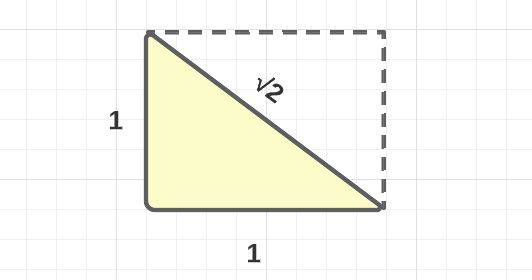
\includegraphics[width = 8cm]{images/crisi_pitagorica.JPG}
    \caption{Teorema del triangolo rettangolo}
    \label{fig:crisi_pitagorica}
\end{figure}

Qualche anno più tardi però la matematica subì un ulteriore arresto con la cosidetta crisi pitagorica.
Tramite il teorema di Pitagorica si riuscì a calcolare la diagonale del quadrato ma, ipotizzando che la figura in questione sia quella \ref{fig:crisi_pitagorica}, il teorema diventa un vero e proprio \textbf{problema}. Perchè essendo $c^2 = a^2 + b^2$ e quindi $c^2 = 2 \rightarrow c = \sqrt{2}$ siamo in difficoltà in quanto non esite un numero razionale che al quadrato dia 2.
\begin{center}
    $\nexists \frac{P}{q} \in \mathbb{Q} :(\frac{P}{q})^2 = 2$
\end{center}

\begin{dimostration}
Possiamo ora procedere per assurdo. Ipotizzando che la tesi sia falsa, ne dedurremmo una contraddizione. Se riusciamo a dimostrare che la tesi non può essere falsa risulterà ovviamente vera.

In questo caso dire che la tesi è falsa significa affermare che $\exists\frac{P}{q}\in\mathbb{Q}:(\frac{P}{q})^2=2$.\\$(\frac{P}{q})^2\Leftrightarrow\frac{P^2}{q^2}=2\Leftrightarrow\frac{P^2q^2}{q^2}=2q^2\Rightarrow q^2$ è pari $\Rightarrow P$ è pari $P=2m, m\in\mathbb{N}$.\\Da $P^2=2q^2$ deriva $(2m^2)=2q^2=4m^2=2q^2\Leftrightarrow2m^2=q^2\Rightarrow q^2$ è pari $\Rightarrow q$ è pari $\Rightarrow q=2m, m\in\mathbb{N}$. Quindi sia $P$ che $q$ sono pari (divisibili per due). Ecco trovata la contraddizione.\flushright{$\blacksquare$}
\end{dimostration}

Da qui nasce la necessità di rappresentare i numeri reali.
\begin{center}
    $\mathbb{R}\{allinamenti\_decimali\_con\_la\_virgola\}$
\end{center}

Si chiamano numeri irrazionali i numeri di $\mathbb{R}\symbol{92}\mathbb{Q}$ come $\sqrt{2}, \pi, e$.

\begin{center}
    \large{Retta dei numeri reali}
\end{center}
\begin{center}
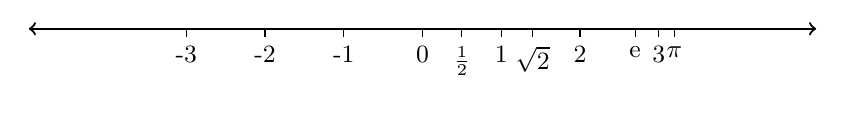
\begin{tikzpicture}
    \draw[<->,thick] (0,0) -- (10,0);
    \draw (5,-0) -- (5,-0.1) node [below] {\small\num{0}};
    \draw (4,-0) -- (4,-0.1) node [below] {\small\num{-1}};
    \draw (3,-0) -- (3,-0.1) node [below] {\small\num{-2}};
    \draw (2,-0) -- (2,-0.1) node [below] {\small\num{-3}};
    \draw (6,-0) -- (6,-0.1) node [below] {\small\num{1}};
    \draw (7,-0) -- (7,-0.1) node [below] {\small\num{2}};
    \draw (8,-0) -- (8,-0.1) node [below] {\small\num{3}};
    \draw (5.5,-0) -- (5.5,-0.1) node [below] {\small{$\frac{1}{2}$}};
    \draw (6.4,-0) -- (6.4,-0.1) node [below] {\small{$\sqrt{2}$}};
    \draw (8.2,-0) -- (8.2,-0.1) node [below] {\small{$\pi$}};
    \draw (7.7,-0) -- (7.7,-0.1) node [below] {\small{e}};
\end{tikzpicture}
\end{center}

\section{Intervalli}

\subsection*{Intervalli limitati}
\begin{definition}[Intervalli limitati]
    Dati $a$ e $b \in \mathbb{R}$ con $a \leq b$, definiamo $[a,b]=\{x\in\mathbb{R}:a\leq x\leq b\}$
\end{definition}

\subsubsection*{Intervalli chiusi}
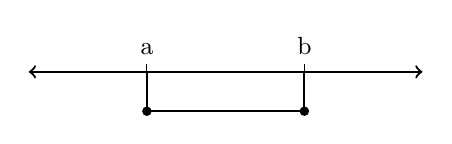
\begin{tikzpicture}
    \draw[<->,thick] (0,0) -- (5,0);
    \draw (1.5,0) -- (1.5,0.1) node [above] {\small{a}};
    \draw (3.5,0) -- (3.5,0.1) node [above] {\small{b}};
    \filldraw[black] (1.5,-0.5) circle (1.5pt);
    \filldraw[black] (3.5,-0.5) circle (1.5pt);
    \draw[-,thick] (1.5,-0.5) -- (3.5,-0.5);
    \draw[-,thick] (1.5,-0) -- (1.5,-0.5);
    \draw[-,thick] (3.5,-0) -- (3.5,-0.5);
\end{tikzpicture}
$]a,b[=\{x\in\mathbb{R}:a\leq x\leq b\}$

\subsubsection*{Intervalli aperti}
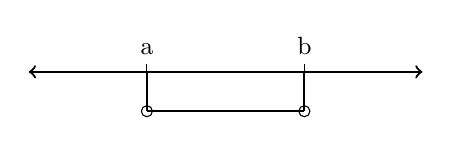
\begin{tikzpicture}
    \draw[<->,thick] (0,0) -- (5,0);
    \draw (1.5,0) -- (1.5,0.1) node [above] {\small{a}};
    \draw (3.5,0) -- (3.5,0.1) node [above] {\small{b}};
    \draw[black] (1.5,-0.5) circle (2pt);
    \draw[black] (3.5,-0.5) circle (2pt);
    \draw[-,thick] (1.5,-0.5) -- (3.5,-0.5);
    \draw[-,thick] (1.5,-0) -- (1.5,-0.5);
    \draw[-,thick] (3.5,-0) -- (3.5,-0.5);
\end{tikzpicture}
$[a,b]=\{x\in\mathbb{R}:a<x<b\}$

Esistono anche altri tipi di intervalli come l'intervallo aperto a sinistra e chiuso a destra, l'intervallo aperto a destra e chiuso a sinistra... ma in tutti i casi i punti $a$ e $b$ vengono sempre chiamati \textbf{estremi dell'intervallo}.

\subsubsection*{Intervalli limitati superiormente e inferiormente}
\begin{definition}
    $\mathbb{A}\subset\mathbb{R}$ si dice superiormente (inferiormente) limitato se $\exists M\in\mathbb{R}(m\in\mathbb{R}):x\leq M(x\geq m), \forall x\in\mathbb{A}$. $M$ è il suo estremo superiore=$\sup(X)$ ($m$ è il suo estremo inferiore=$\inf(X)$).
\end{definition}

\subsection*{Intervalli illimitati}
Dato $a$ in $\mathbb{R}$ si definiscono intervalli illimitati i seguenti periodi:\\ $]-\infty,a],\hspace{0,5cm}]-\infty,a[,\hspace{0,5cm}[a,+\infty[,\hspace{0,5cm}]a,+\infty[,\hspace{0,5cm}\mathbb{R}=]-\infty,+\infty[=\{x\in\mathbb{R}\}$

\subsection*{Modulo e valore assoluto}
Dato $r\in\mathbb{R}$ definisco 
\begin{equation}
|r|=\begin{cases}
r, se, r\geq 0\\
-r, se, r<0
\end{cases}
\end{equation}

$|5|=5\hspace{0.5cm}|-5|=-(-5)=5$

Il modulo serve per calcolare la distanza tra due numeri. Dati $a$ e $b\in\mathbb{R}$, la loro distanza è definita come $|a-b|$ oppure $|b-a|$.
\subsubsection*{Disuguaglianza triangolare}
Con la disuguaglianza triangolare affermiamo che una somma in valore assoluto è sempre maggiore o uguale ai due numeri in valore assoluto sommati separatamente.
\begin{center}
    $|x+y|\leq |x|+|y|\hspace{0.5cm}\forall x,y\in\mathbb{R}$
\end{center}
Vale anche per $|\sum_{i=1}^{n}x_1|\leq\sum_{i=1}^{n}|x_2|$.

\subsection*{Massimi e minimi}
\begin{definition}[Massimi e minimi]
    Dato $\mathbb{A}\subset\mathbb{R}$, se $\exists M\in\mathbb{A}:M\geq x, \forall x\in\mathbb{A}$, allora $M$ si chiama massimo di $A$.
    Dato $\mathbb{A}\subset\mathbb{R}$, se $\exists m\in\mathbb{A}:m\leq x, \forall x\in\mathbb{A}$, allora $m$ si chiama minimo di $A$.
\end{definition}
\begin{center}
    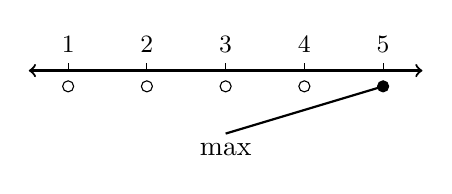
\begin{tikzpicture}
        \draw[<->,thick] (0,0) -- (5,0);
        \draw (0.5,0) -- (0.5,0.1) node [above] {\small{1}};
        \draw (1.5,0) -- (1.5,0.1) node [above] {\small{2}};
        \draw (2.5,0) -- (2.5,0.1) node [above] {\small{3}};
        \draw (3.5,0) -- (3.5,0.1) node [above] {\small{4}};
        \draw (4.5,0) -- (4.5,0.1) node [above] {\small{5}};
        \draw[black] (0.5,-0.2) circle (2pt);
        \draw[black] (1.5,-0.2) circle (2pt);
        \draw[black] (2.5,-0.2) circle (2pt);
        \draw[black] (3.5,-0.2) circle (2pt);
        \filldraw[black] (4.5,-0.2) circle (2pt);
        \draw (2.5,-1.2) -- (2.5,-1.2) node [above] {\normalsize{max}};
        \draw[-,thick] (2.5,-0.8) -- (4.5,-0.2);
    \end{tikzpicture}\hspace{1cm}
    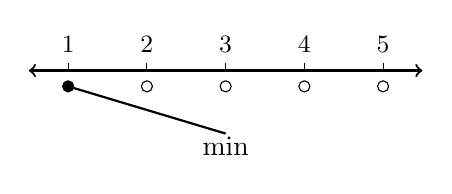
\begin{tikzpicture}
        \draw[<->,thick] (0,0) -- (5,0);
        \draw (0.5,0) -- (0.5,0.1) node [above] {\small{1}};
        \draw (1.5,0) -- (1.5,0.1) node [above] {\small{2}};
        \draw (2.5,0) -- (2.5,0.1) node [above] {\small{3}};
        \draw (3.5,0) -- (3.5,0.1) node [above] {\small{4}};
        \draw (4.5,0) -- (4.5,0.1) node [above] {\small{5}};
        \filldraw[black] (0.5,-0.2) circle (2pt);
        \draw[black] (1.5,-0.2) circle (2pt);
        \draw[black] (2.5,-0.2) circle (2pt);
        \draw[black] (3.5,-0.2) circle (2pt);
        \draw[black] (4.5,-0.2) circle (2pt);
        \draw (2.5,-1.2) -- (2.5,-1.2) node [above] {\normalsize{min}};
        \draw[-,thick] (2.5,-0.8) -- (0.5,-0.2);
    \end{tikzpicture}
\end{center}
Può accadere inoltre che un'intervallo non abbia un punto di massimo o di minimo o entrambe $]1,2[$.

\section{Radicali, potenze, logaritmi}

\subsection*{Radici n-esime}
Se voglio calcolare la radice di 2 posso, con le conoscenze apprese, trovare i numeri per approssimazione. Questo procedimento, anche se giusto, risulta enormemente inefficiente.

In generale posso quindi calcolare $x^{\frac{P}{q}}, \forall x^{\frac{P}{q}}\in \mathbb{Q}$, scrivendolo come:
\begin{equation}
    (\sqrt[q]{x})^P=(x^{\frac{1}{q}})^P
\end{equation}

\subsection*{Potenze}\label{sec:proprieta_potenze}
Le proprietà principali delle potenze sono le seguenti:
\begin{equation}
    a^0=1\hspace{0,5cm}0^r=1\hspace{0,5cm}0^0=\nexists
\end{equation}
\begin{equation}
    a^r*a^s=a^{r+s}
\end{equation}
\begin{equation}
    a^r*b^r=(ab)^r
\end{equation}
\begin{equation}
    (a^r)^s=a^{rs}
\end{equation}
\begin{equation}
    a^{-r}=\frac{1}{a^r}
\end{equation}

\subsection*{Logaritmi}
$\forall x,y\in\mathbb{R}, a^x=y,\log_{a}{y}=x\Rightarrow a^x=y$.

Il logaritmo è la funzione inversa dell'esponenziale.

La base del logaritmo può assumere due valori diversi: $a>1$ e $0<a<1$. A seconda del valore della base cambia anche il suo grafico.
\begin{figure}[ht]
    \centering
    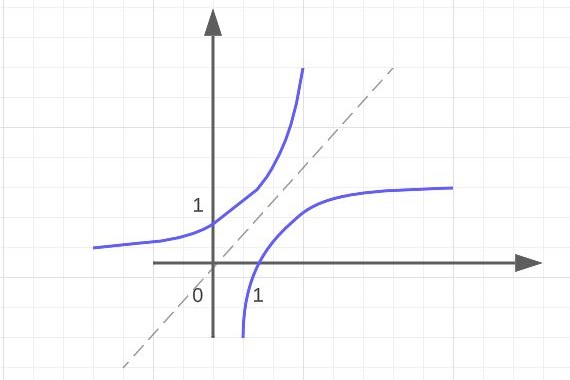
\includegraphics[width = 5.8cm]{images/log_1.JPG}\quad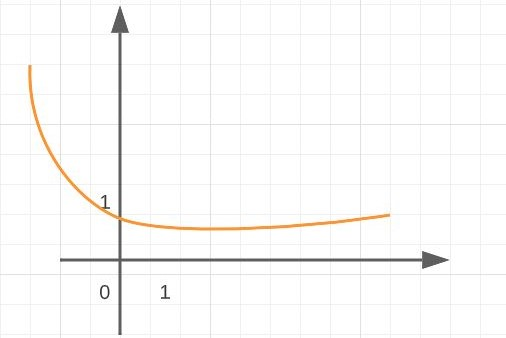
\includegraphics[width = 5.8cm]{images/log_01.JPG}
    \caption{Grafici dei logaritmi in base $a>1$ e $0<a<1$}
    \label{fig:log}
\end{figure}

\subsubsection*{Proprietà dei logaritmi}
Anche i logritmi hanno le proprie propietà. Essendo il logaritmo per definizione l'inverso dell'esponenziale, è necessario un ripasso delle proprietà delle potenze nella sezione \ref{sec:proprieta_potenze}.

Prendiamo quindi i valori $a>0$ e $a\neq 1$
\begin{equation}
    a^{\log_{a}{x}}=x\hspace{0,5cm}\log_{a}{a^x}=x\hspace{0,5cm}\log_{a}{a}=1
\end{equation}
\begin{equation}
    \log_{a}{1}=0
\end{equation}
\begin{equation}
    \log_{a}{x*y}=\log_{a}{x}+\log_{a}{y}
\end{equation}
\begin{equation}
    \log_{a}{x^\alpha}=\alpha\log_{a}{x}\hspace{0,5cm}\forall\alpha\in\mathbb{R}
\end{equation}
\begin{equation}
    \log_{a}{\frac{1}{x}}=\log_{a}{x^{-1}}=-\log_{a}{x}
\end{equation}
\begin{equation}
    \log_{a}{\frac{x}{y}}=\log_{a}{x}-\log_{a}{y}
\end{equation}
\begin{equation}
    \log_{a}{x}=\frac{\log_{b}{x}}{\log_{b}{a}}\hspace{0,5cm}\forall a,b>0, a,b\neq 1, x>0
\end{equation}

\subsubsection*{Logaritmo naturale}
$\ln{x}=\log_{e}{x}\hspace{0,5cm}e\simeq 2,7$

\section{Equzioni e disequazioni}

\subsection*{Polinomi}
\begin{definition}
    Un polinomio è un espressione del tipo $P(x)=a_0x^0+a_1a^1+a_2a^2+...+a_nx^n$.
\end{definition}
\begin{equation}
    \sum_{i=0}^{n}a_i*n^i\hspace{0,5cm}a_0,...,a_n\in\mathbb{R}
\end{equation}
A volte i polinomi possono anche essere fattorizzati.
\begin{example}
    $x^3+x^2-x-1\hspace{0,5cm}x^2(x+1)-(x+1)\hspace{0,5cm}(x^2-1)(x+1)\hspace{0,5cm}(x+1)(x-1)(x+1)\hspace{0,5cm}(x+1)^2(x-1)$
\end{example}

\subsection*{Equazioni}
\begin{definition}
    Un'equazione è un uguaglianza con una variabile incognita.
\end{definition}
Per risolvere l'identità, vogliamo calcolare la $x$ che la rende vera.

\subsubsection*{Equazioni lineari o di primo grado}
\begin{example}\label{es:eq_lineare}
    $2x-5=7$
\end{example}
Per risolvere l'esempio \ref{es:eq_lineare} dobbiamo trovare tutte le $x\in\mathbb{R}$ tali che $2x-5=7$. A tal punto effettuiamo delle manipolazioni algebriche.

\begin{tabular}{c m{3cm} m{3cm}}
     $2x-5=7\Rightarrow$ & $2x=7+5\Rightarrow$ & $x=6$.\\
     & \textit{Sommo 5 a sinistra e a destra.} & \textit{Divido per 2 a sinistra e a destra.}
\end{tabular}

\subsubsection*{Equazioni di secondo grado}
Un'equazione di secondo grado è un'uguaglianza scritta nella forma:
\begin{equation*}
    ax^2+bx+c=0
\end{equation*}
Le equazioni di secondo grado comportano l'aggiunta di qualche passaggio extra.
Le soluzioni si calcolano con la formula:
\begin{equation}
    x_{1,2}=\frac{-b\pm\sqrt{b^2-4ac}}{2a}
\end{equation}
\begin{center}

    $\Delta =b^2-4ac$\hspace{1cm}
    \begin{tabular}{c|c}
         $\Delta =0$ & due soluzioni reali e coincidenti\\\hline
         $\Delta >0$ & due soluzioni reali e distinte\\\hline
         $\Delta <0$ & non esistono soluzioni
    \end{tabular}
\end{center}
\begin{example}\label{es:eq_2gr}
    $x^2-3x+2=0\hspace{0,5cm}x_{1,2}=\frac{3\pm\sqrt{9-8}}{2a}\hspace{0,5cm}x_{1,2}=\frac{3\pm 1}{2}$\hspace{0,5cm} Soluzioni $2$ e $1$.
    
    Infatti se verifichiamo inserendo i valori nell'equazione di partenza l'identità è risolta.
\end{example}

\subsubsection*{Equazioni con valore assoluto}
Consideriamo il seguente poliniomio $|A(x)|=k, k\in\mathbb{R}$ e distinguiamo diversi casi:
\begin{enumerate}
    \item Se $k>0$ equivale all'unione degli insiemi $A(x)=k$ e $A(x)=-k$;
    \item Se $k=0$, $A(x)=0$;
    \item Infine se $k<0$ non ammette soluzioni perchè equivale a confrontare un termine negativo con uno sempre positivo.
\end{enumerate}

\subsection*{Disequazioni}
Le disequazioni sono simili alle equazioni ma con $<,\leq,>,\geq$ al posto di $=$.
Al contrario delle equazioni però, le disequazioni esprimono il loro risultato in intervalli.
\begin{example}
$5-8x>13$
\begin{center}
\begin{tabular}{m{3cm} m{3cm} m{3cm}}
     $-8x>13-5\Rightarrow$ & $8x<-8\Rightarrow$ & $x<-1$\\
     Sommo per -5 a sinistra e a destra. & Cambio il verso della disequazione. & Divido per 8 a destra e a sinistra.
\end{tabular}
\end{center}

L'equazione è verificata per tutti i valori di $x<-1$. In intervallo $]-\infty,-1[$
\end{example}

\subsubsection*{Disequazioni di secondo grado}
Il grafico di una disequazione di secondo grado è una parabola rivolta verso l'alto se $a>0$, verso il basso se $a<0$.
\begin{example}
    $x^2-3x+2\leq 0$
    
    Come prima cosa risolviamo l'equazione associata come nell'esercizio \ref{es:eq_2gr}. $x^2-3x+2=0$ le cui soluzioni sono: $2$ e $1$.
    Una volta trovati i valori facciamo riferimento alla seguente tabella per rappresentare l'intervallo delle soluzioni con $a>0$:
\begin{table}[h]
    \centering
    \begin{tabular}{|c|c|c|c|c|}
        \hline$\Delta$ & $>$ & $\geq$ & $<$ & $\leq$\\\hline\hline
        $\Delta >0$ & $x<x_1 \vee x>x_2$ & $x\leq x_1 \vee x\geq x_2$ & $x_1<x<x_2$ & $x_1\leq x\leq x_2$\\\hline
        $\Delta <0$ & $\forall x\in\mathbb{R}$ & $\forall x\in\mathbb{R}$ & $\nexists x\in\mathbb{R}$ & $\nexists x\in\mathbb{R}$\\\hline
        $\Delta =0$ & $x\neq x_1$ & $\forall x\in\mathbb{R}$ & $\nexists x\in\mathbb{R}$ & $x=x_1$\\\hline
    \end{tabular}
    \caption{Tabella dello studio del segno}
    \label{tab:eq_2gr_sds}
\end{table}
\end{example}

\subsubsection*{Disequazioni con valore assoluto}
A differenza delle disequazioni precedenti, per risolvere una disequazione in valore assoluto, indipendentemente dal suo segno, possiamo impostare la soluzione come l'unione di due sistemi. Quindi data la disequazione $|f(x)|\gtrless c, c>0$ la sua soluzione sarà data da:

\begin{center}
    \[
  \begin{cases}
    f(x)\geq 0 \\
    f(x)\gtrless c
    
  \end{cases}
  \begin{cases}
       f(x)<0\\
       -f(x)\gtrless c
  \end{cases}
  \]
\end{center}
          
\subsection*{Grado superiore al secondo}
\subsubsection*{Variabile t}
Se successivamento alle nostre scomposizione ci troviamo ancora difronte a una equazione/disequazione di grado superiore al secondo, possiamo porre ad esempio $x^2=t$ e calcolare le nostre soluzioni per t.
Una volta trovate le soluzioni non resta che trasformare di nuovo in $t=x^2$.

\subsubsection*{Ruffini}
Se anche con il metodo precedente non riusciamo nel nostro intento, possiamo sempre applicare Ruffini.

Come prima cosa dobbiamo trovare un valore che messo al posto della x faccia risultare l'equazione uguale a 0. Successivamente scriviamo in tabella i coefficienti dei termini. Eseguiamo le sottrazioni e moltiplicazioni e assicuriamoci che il risultato sia ancora 0.
A questo punto non resta che scrivere la nostra nuova equazione semplificata.
\begin{example}
    $x^3-2^2-5x+6=0$
    \begin{center}
        \begin{tabular}{c|ccc|c}
            &1&-2&-5&6\\
            1&&1&1&-6\\\hline
            &1&-1&-6&0\\
        \end{tabular}
    \end{center}
    $(x-1)(1x^2-1x-6)=0$
\end{example}


\section{Binomio di Newton}\label{sec:binomio_Newton}
Vogliamo calcolare la potenza del binomio dei primi $n$ numeri:

$(a+b)^0=1\\(a+b)^1=a+b\\(a+b)^2=a^2+2ab+b^2\\(a+b)^3=a^3+3a^2b+3ab^2+b^3\\(a+b)^4=\text{ diventa più complesso}$

Proprio per questo motivo è stato sviluppato quello che viene chiamato binomio di Newton, che ci permette di calcolare il binomio elevato a qualsiasi potenza.
\begin{equation*}
    (a+b)^n=(a+b)(a+b)\text{ n volte }=c_na^n+c_na^{n-1}+\text{ ... }+c_nb^n
\end{equation*}
Il coefficiente $c_{\frac{n}{k}}a^{n-k}b^n$ corrisponde al numero di possibili combinazioni dei $k$ elementi. Questo numero è anche chiamato coefficiante binomiale:
\begin{equation}
    \binom{n}{k}=\frac{n!}{k!(n-k)!}
\end{equation}

\begin{example}
    Coefficiente binomiale di $(a+b)^4$.
    
    $(a+b)^4=\binom{4}{0}a^4+\binom{4}{1}a^3b+\binom{4}{2}a^2b^2+\binom{4}{3}ab^3+\binom{4}{4}b^4$
\end{example}

\subsection*{Triangolo di Tartaglia}
Il triangolo di Tartaglia serve per calcolare i coefficienti di $a$ e $b$ in elevazioni binomiali.

Il triangolo è formato nel vertice e lungo i lati dalla cifra 1 e le altre cifre sono data dalla somma delle due della riga superiore.

\begin{table}[ht]
    \centering
    \begin{tabular}{c|ccccccccccc}
        0& &&&&&1&&&&&\\
        1& &&&&1&&1&&&&\\
        2& &&&1&&2&&1&&&\\
        3& &&1&&3&&3&&1&&\\
        4& &1&&4&&6&&4&&1&\\
        5& 1&&5&&10&&10&&5&&1\\
    \end{tabular}
    \caption{Triangolo di tartaglia}
    \label{tab:tr_tart}
\end{table}

Ad esempio se vogliamo calcolare $(a+b)^4$ avremo, guardando la Tabella \ref{tab:tr_tart}, $a^4+3a^3b+6a^2b^2+4ab^3+b^4$.